\documentclass[../598comp.tex]{subfiles}

\date{05-13}

\begin{document}

\section{05-13}

\subsection{Bisimulation}

Transition systems as models of software or hardware or embedded systems.

Nondeterminism, need not be finite state.

When are two systems observably the same?


\begin{example}[Vending Machine]
  Difference from DFA, some actions get rejected. The rejection is different
  from the rejection in an NFA because really that encodes a state where you
  can't escape, while this is more true rejection. No start states or accept
  states. Just interested in what actions we see.
  \\
  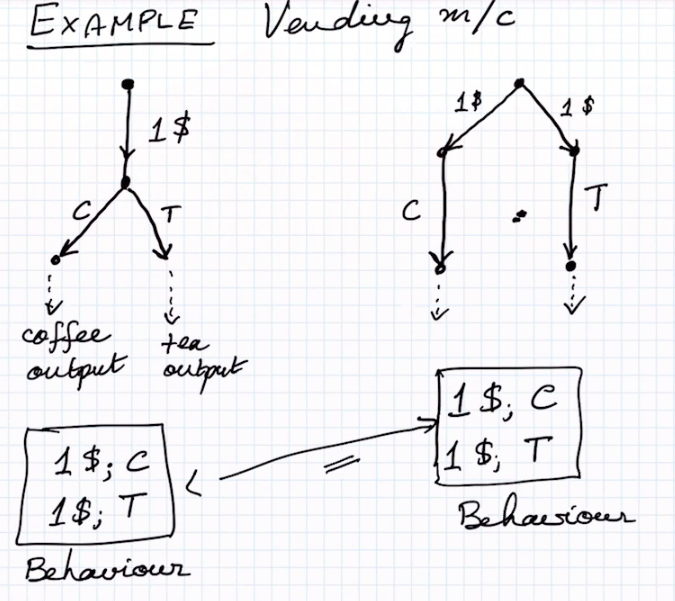
\includegraphics[width=\textwidth]{vending_machine}
  \\
  Internal vs. external choice is what makes these two machines different. This
  shows how sequences are inadequate description of the behavior. So how can we
  actually compare to LTS? With bisimulation.
\end{example}

\begin{definition}[LTS (Labeled Transition System)]
  \begin{gather*}
    S \to \ \text{set of states, perhaps infinite} \\
    A \to \ \text{set of actions, finite} \\
    \to \subseteq S \times A \times S \\
    (s, a, s') \in \to, \quad s \overset{a}{\to} s'
  \end{gather*}
  From state $s$, if action $a$ is performed, you can end up in $s'$.
\end{definition}

\begin{definition}[Bisimulation (semi-formed)]
  When comparing two systems, we form a binary relation between the states of a
  simple. This isn't a big deal because we could merge the two systems.
  \\\\
  We say $s, t \in S$ are \ul{bisimilar} (written $s \sim t$) if 
  \begin{gather*}
    \forall a \in A \ s \overset{a}{\to} s' \Rightarrow \exists t' s.t. t
    \overset{a}{\to} t' \ \text{and} \ s' \sim t' \\
    \forall a \in A t \overset{a}{\to} t' \Rightarrow \exists s' s.t. s
    \overset{a}{\to} s' \ \text{and} \ s' \sim t'
  \end{gather*}
  If $s$ can do something, $t$ can do the same thing. And they may end up in
  different states, but those states themselves will be bisimilar. This should
  make you uneasy because it's an inductive definition with no base case.
  \\\\
  There are 4 ways of clarifying this definition.
  \begin{enumerate}
  \item 
    We define an $\NN$ indexed family of equivalence relations (infinitely many
    of them) as follows: $s \sim_0 t$ always. Then
    \begin{gather*}
      s \sim_{n + 1} \ if \ \forall a \in A \ s \overset{a}{\to} s' \Rightarrow \exists t' s.t. t \overset{a}{\to} t' \ \text{and} \ s' \sim_n t' \\
      \text{vice versa}
    \end{gather*}
    Now we say that $\sim = \cap_n \sim_n$
    \\\\
    In the vending machine example $s_0 \sim_1 t_0$ but $s_0 \not\sim_2 t_0$ and
    hence they are certainly not bisimilar systems.
  \item
    $R$ the family of equivalence relations $\subseteq S \times S$ order by
    inclusion. Smallest is everything is related to itself. Largest is
    everything related to everything. This forms a complete lattice. $F: R \to
    R$.
    \begin{gather*}
      s F(R) t \ \text{if} \ \forall a s \overset{a}{\to} s' \Rightarrow \exists
      t' s.t. t \overset{a}{\to} t' \ \text{and} \ s' R t' \\
      \text{vice versa}
    \end{gather*}
    $F$ is easily seen to be monotone i.e. if $R_1 \subseteq R_2$ then $F(R_1)
    \subseteq F(R_2)$. It follows that there is a unique greatest fixed point.
    i.e. a special $\sim \in R$ such that $F(\sim) = \sim$ and if $R$ is any
    relatoin such that $F(R) = R$ then $R \subseteq \sim$. This is called fixed
    point bisimilarity. 
  \item
    We saw $R$ is a dynamic relation or a bisimulation relation if whenever
    $sRt$ then .
    \begin{gather*}
      \forall a \forall s' \ s \overset{a}{\to} s' \Rightarrow \exists t' s.t. t
      \overset{a}{\to} t' \ \text{and} \ s'Rt' \\
      \text{vice versa}
    \end{gather*}
    Note that this is not circular. $R$ is given somehow and it may or may not
    have this property. We say that $s \sim t$ if $\exists R$, a bisimulation
    relation with $sRt$.
    \begin{fact}
      If $R_i$ is any family of bisimulation relations, then $\cup_iR_i$ is also
      a bisimulation as is $\cap_iR_i$. $\sim = \cup_{R_a}R$.
    \end{fact}
    Easy to see that (2) and (3) are equivalent. (1) is \ul{not} equivalent
    without a further assumption.
  \end{enumerate}
\end{definition}

\subsection{Lattice Theory and Fixed Points}

Remember that a poset is a partially ordered set. i.e. a set equipped with a
partial order.
\\\\
Given $(S, \leq)$, we say that $u$ is \ul{the least upper bound} of $X \subseteq
S$ if 
\begin{gather*}
  \forall x \in X, \ x \leq u \ \text{and} \ \forall y \in S, if \ \forall x \in X, x
  \leq y \Rightarrow u \leq y
\end{gather*}
If $X \subseteq S$ we say $v$ is a lower bound of x if $\forall x \in X, \ v
\leq x$. If $v$ in addition is greater than any other lower bound, we call it
the Infimum.
\begin{definition}
  In a lattice there is a supremum and infimum for \ul{every pair} of elements.
  They are not necessarily unique. By induction it follows that every finite set
  of elements has a supremum and infimum. Infinite numbers may not.
\end{definition}
\begin{definition}[Complete Lattice]
  A lattice is complete if every subset has a least upper bound.
  \begin{fact}
    It follows that every set has a greatest lower bound.
  \end{fact}
\end{definition}
The least upper bound of $\varnothing$ is a least element of the whole set.
\begin{proof}
  Let $X \subseteq L$, where $L$ is a complete lattice. Let $V = \{v \in L \ | \
  \forall x \in X \ v \leq x\}$ be the set of lower bounds of $X$.
  \\\\
  Let $g = \sup(V)$. Claim $g$ is $\inf(X)$.
  \begin{note}
    $\forall x \in X, \ \forall v \in V, \ v \leq x$. i.e. $\forall x \in X$,
    $x$ is an upper bound for $V$ so since $g$ is the lesat upper bound for $V$
    we have that $\forall x \in X, \ g \leq x$, i.e. $g \in V$.
    \\\\
    Since $g$ is an upper bound for $V$ it is greatre than any element of $V$ so
    it is the glb of $X$.
  \end{note}
\end{proof}
\begin{theorem}
  If $f: L \to L$ is monotone and $L$ is a complete lattice, then the fixed
  points of $f$, i.e. $x \ s.t.\ f(x) = x$ forms a complete lattice in its own
  right. In particular there is a least fixed point and a greatest fixed point.
  There is a least fixed point and a greatest fixed point.
  \begin{proof}
    Find the upper bound of set of inflationary points and show that it is fixed.
  \end{proof}
\end{theorem}
Note to be a bisimulation relation means $R \subseteq F(R)$. Least upper bound
of $\{R \ | \ R \ \text{is a bisimulation}\} = \cup_{R}R = gfp(F)$ (greatest
fixed point).
(2) and (3) are really the same. (1) is not the same unless the transition
system has a special property $\forall s, a \{t \ | s \to_a t\}$ is finite.
This is called image-finiteness.
\\\\
If TS is image finite then (1) is equivalent to (2) and (3). The definition of
bisimulation is an example of a co-inductive definition.
% revisit coinduction

\subsection{Logical Characterization of Bisimulation}

Given an LTS, we define a \ul{modal} logic called Hennessy-Milner Logic.
\begin{gather*}
  \varphi ::== T \ | \ \neg \varphi \ | \ \varphi_1 \wedge \varphi_2 \ | \
  \langle  a \rangle \varphi 
\end{gather*}
$s \models \langle  a \rangle \varphi \rangle$ if $\exists t \ s.t. \ s \to_a t$
and $t \models \varphi$. At least one state satisfies.
\\\\
$[a]\varphi = \neg \langle  a \rangle \neg \varphi$
\\\\
Every state $t$ such that $s \to_a t$ must satisfy $\varphi$.

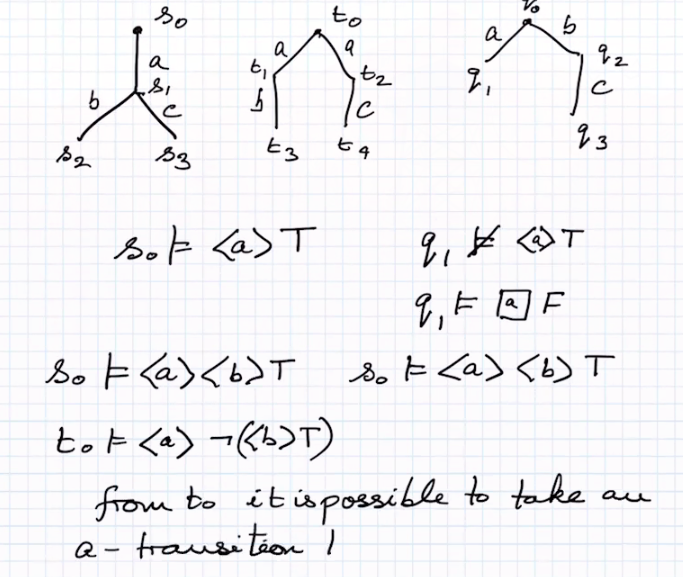
\includegraphics[width=\textwidth]{transitionsbi.png}
\begin{theorem}
  $s \sim t$ if and only if $\forall \varphi s \models \varphi \iff t \models
  \varphi$ (image finiteness assumed). Don't be afraid of infinite conjunctions.
  \begin{proof}
    We define a new equivalence relation $\approx$. $s \approx t \iff \forall
    \varphi \ s \models \varphi \iff t \models \varphi$.
    \\\\
    Idea is to prove that $\approx$ is a bisim relation. Suppose $s \approx t$
    and suppose $s \to_a s'$. We want to show that $\exists t' \ s.t. t \to_a
    t'$ and $s' \approx t'$.
    \\\\
    Assume that $s$ and $t$ are not bisimilar. Then $\forall t' \ s.t. \ t \to_a
    t'$, $s' \not \approx t'$. There are only finitely many such $t': t'_1,
    \dots, t'_n$. % review
  \end{proof}
\end{theorem}

\subsection{Probabilistic Bisimulation and Logical Characterizaiton}

Probabilistic transition systems. $s \models \langle a \rangle_q \varphi$. $a
\in Act, \ q \in Q \cap [0, 1]$
The probability of winding up in a state sastisfying $\varphi$ after doing an
$a$ action in state $s \geq q$. Larsen and Skou proved logical characterization
using
\begin{gather*}
  \langle a \rangle_q \varphi \ \text{and} \ \neg \varphi \ \text{and} \
  \varphi_1 \wedge \varphi_2
\end{gather*}
They also assumed a very strong finite branching property. And probabilities
must be integer multiples of some fixed rational number.
\\\\
AMAZINGLY proved logical characterization with no finite branching assumption
and no negation in the logic. We alo got logical characterization of simulation.




\end{document}